\documentclass[12pt]{article}

\usepackage{amsmath}
\usepackage[authoryear,round]{natbib}
%\usepackage{hyperref}

\textwidth=6.2in
\textheight=8.5in
\oddsidemargin=.1in
\evensidemargin=.1in
\headheight=-.3in

\newcommand{\scscst}{\scriptscriptstyle}
\newcommand{\scst}{\scriptstyle}
\newcommand{\Rfunction}[1]{{\texttt{#1()}}}
\newcommand{\Rmethod}[1]{{\texttt{#1}}}  
\newcommand{\Rclass}[1]{{\texttt{#1}}}
\newcommand{\Robject}[1]{{\texttt{#1}}}
\newcommand{\Rpackage}[1]{{\textit{#1}}}
\newcommand{\code}[1]{{\texttt{#1}}}
\bibliographystyle{plainnat}
\def\tm{$^{\rm \text{TM }}$}

\title{Analysis of High Throughput Flow Cytometry Data using
\Rpackage{plateCore}}

%%%%%%%%%%%%%%%%%%%%%%%%%%%%%%%%%%%%%%%%%%%%%%%%%%%%%%%%%%%%%%%%%%%%%%%%%%%
\usepackage{Sweave}
\begin{document}
\maketitle

\clearpage
%%%%%%%%%%%%%%%%%%%%%%%%%%%%%%%%%%%%%%%%%%%%%%%%%%%%%%%%%%%%%%%%%%%%%%%%%%%%%%
\section*{Abstract}
\subsection*{Background}
High throughput flow cytometry (FCM) studies are often run in a 96 or 384-well
plate format, with different samples, controls, and antibodies-dye conjugates
present on each plate. Analyzing a plate requires tracking the contents of each
well, matching sample wells with control wells, gating each well/channel
separately, making the appropriate plots, assessing quality, and finally
aggregating the results from multiple plates to make experiment level
conclusions. This process can be a significant task using traditional
point-and-click software packages, even when multiple instances are deployed.
We developed \Rpackage{plateCore} as an R/Bioconductor packaged to make
processing and analysis of large, complex datasets easier.

\subsection*{Methods}
\Rpackage{plateCore} was used to analyze the data from a BD FACS CAP screening
experiment where 5 Peripheral Blood Mononucleocyte Cell (PBMC) samples  were
assayed for 189 different human cell surface markers. This same dataset was
also manually analyzed by a cytometry expert using the FlowJo data analysis
software package (TreeStar, Ashland OR).

\subsection*{Results}
Positive markers identified using \Rpackage{plateCore} are in good agreement
with those found using manual analysis.

\subsection*{Conclusions}
\Rpackage{plateCore} provides a reproducible, objective platform for analyzing
high throughput FCM experiments. The R/Bioconductor implementation allows
bioinformaticians and statisticians access to the data, which should further
the development of automated analysis methods.

\clearpage
%%%%%%%%%%%%%%%%%%%%%%%%%%%%%%%%%%%%%%%%%%%%%%%%%%%%%%%%%%%%%%%%%%%%%%%%%%%%%%%
\section*{Introduction}

While there are a number of different software packages available for analysis
of FCM data, these programs are often ill-suited to the development of new
methods needed for analyzing high-throughput FCM studies. Flow Cytometry High
Content Screening (FC-HCS) experiments generate large volumes of data, and a
systematic approach to preprocessing, gating (i.e. filtering), and summarizing
results is needed for robust analyses. Automation of these steps would allow
analysis pipelines to be robust, objective, and match the high-throughput
capacity of modern cytometers. Unfortunately, current approaches to FC-HCS
analysis are semi-automated at best, and they often require significant
subjective and error-prone manual intervention to identify cells of interest
\citep{Maecker2005}. It is therefore desirable to develop programmatic
approaches to process FCM data.

FCM packages available through the Bioconductor \citep{BIOC} project provide an
open platform that can be used by cytometrists, bioinformaticians, and
statisticians to collaboratively develop new methods for automated FC-HCS
analysis. The basic data processing tools for importing, transforming, gating,
and organizing raw FCM data are in the \Rpackage{flowCore} package
\citep{hahne2009}, and the visualization functions are in \Rpackage{flowViz}
\citep{sarkar2008ufv}. The Bioconductor model for FCM data analysis facilitates
the development of new analysis methods, since the overhead associated with
accessing and visualizing FCM data is handled by \Rpackage{flowCore} and
\Rpackage{flowViz}. The availability of \Rpackage{flowCore} and
\Rpackage{flowViz} has enabled the creation of new tools for quality assessment
of large FCM experiments, such as \Rpackage{flowQ} \citep{lemeurFQ}, and
model-based clustering and automated gating, such as \Rpackage{flowClust}
\citep{lo2008}.

We have developed an R package (\Rpackage{plateCore}) that also takes advantage
of the functionality in \Rpackage{flowCore} and \Rpackage{flowViz} to create
methods and data structures for processing large, plate-based FCM datasets.
\Rpackage{plateCore} is not designed to be a GUI driven end-user tool, but
rather to help develop a standardized platform for the analysis of FC-HCS data.
These analyses often represent a collaborative effort between cytometry experts
who generate the data and the quantitative individuals who help deal with the
large volume information. In order for this collaboration to work, the
cytometrists must have confidence in the results of the automated analysis. To
this point, we demonstrate the equality of our results to those produced by an
expert cytometrist using FlowJo.

\begin{figure}
\centering
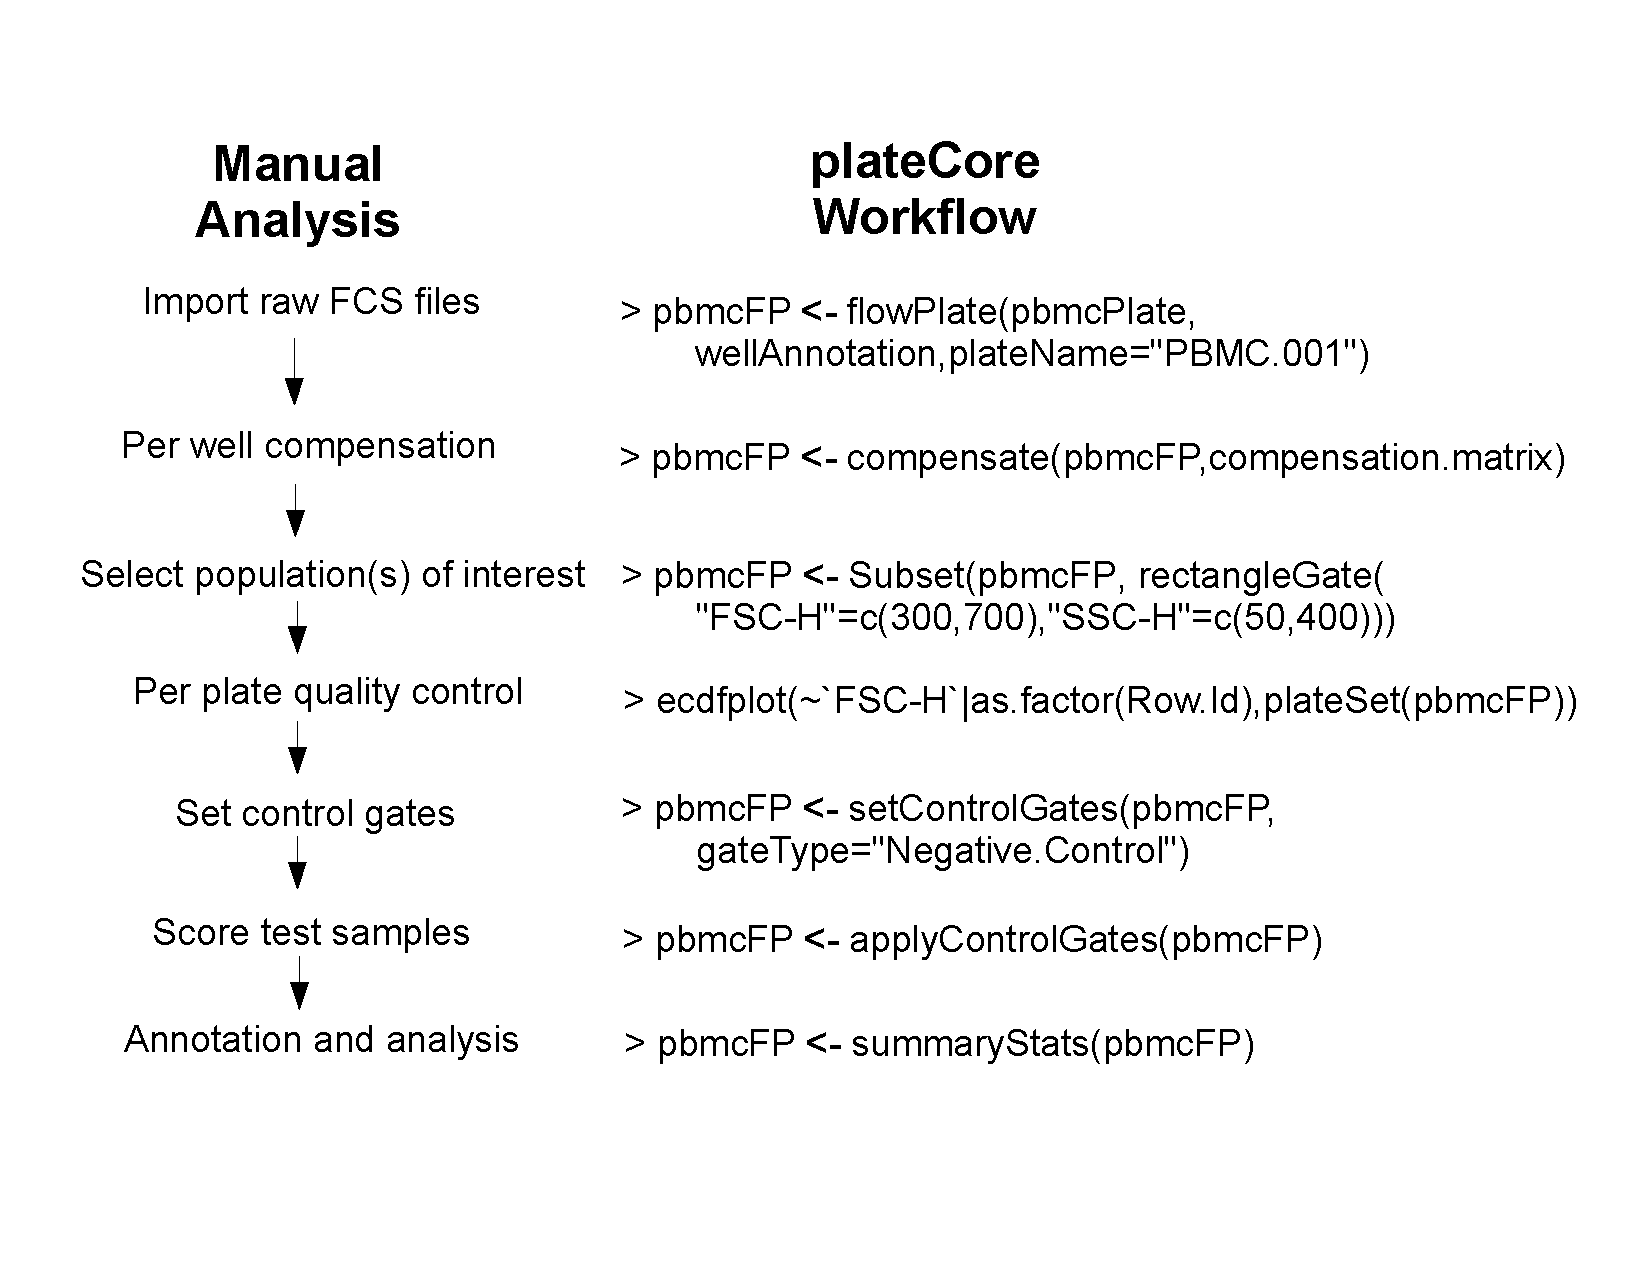
\includegraphics[width=7in,height=6in]{analysisSteps.pdf}
\caption{Typical FC-HCS plate workflow on the left and corresponding steps from
a PBMC lymphocyte \Rpackage{plateCore} analysis on the right. Compared to
analyses performed using existing GUI FCM tools, \Rpackage{plateCore} can
reduce the level of subjectivity associated with creating the negative control
gates and also makes it easier to aggregate multiple plates into an experiment
level object for visualization and reporting. Providing \Rpackage{plateCore}
scripts along with the raw FCM data for FC-HCS experiments helps to ensure that
analysis is transparent and reproducible.}
\label{fig:analysis}
\end{figure}
 
%%%%%%%%%%%%%%%%%%%%%%%%%%%%%%%%%%%%%%%%%%%%%%%%%%%%%%%%%%%%%%%%%%%%%%%%%%%%%%%%
\clearpage
\section*{Materials and Methods}
\subsection*{Flow Cytometry Data}

The data analyzed in this study was part of the initial set of experiments
used to validate the BD FACS CAP platform. BD FACS CAP was designed as a cell
characterization tool to screen for the presence of a large number of different
human cell surface markers, and it was important to show that the assay was
able to correctly identify positive and negatively staining markers on a well
studied cell population, such as PBMC lymphocytes. Previously
frozen PBMC samples from two donors were analyzed on a BD FACS Calibur using BD
FACS CAP staining plates. The analysis was performed on 96-well plates with 189
different antibodies arrayed three per well in 63 test wells, along with 30
isotype control wells and three unstained controls. The complete list of BD
FACS CAP antibodies can be found at
http://www.bd.com/technologies/discovery\_platform/BD\_FACS\_CAP.asp. FCM files
for the 5 plates (two for Donor 1 and three for Donor 2), are available for
download from http://www.ficcs.org.

%%%%%%%%%%%%%%%%%%%%%%%%%%%%%%%%%%%%%%%%%%%%%%%%%%%%%%%%%%%%%%%%%%%%%%%%%%%%%%%%
\subsection*{\Rpackage{plateCore}}

The \Rpackage{plateCore}
scripts used to perform the analysis are provided in supplementary materials.
Briefly, the FCM files were first processed using a combination of static
gates(\Robject{rectangleGate}) and data driven gates (using
\Robject{norm2filter} and \Rpackage{flowCore}) to pick out the lymphocytes in
the forward (FSC) and side scatter (SSC) channels.  The
quality of the data was then assessed by looking for fluidic events such as
bubbles, pressure drops, or large aggregates that can shift the baseline
fluorescence readings. Fluidic events can often be identified by plotting the
empirical cumulative density (ecdf) plots of FSC values for each well, and
looking for distributions shifted relative to other wells \citep{lemeur2007}.
Based on the ecdf plots, several wells were further investigated by cytometry
experts who determined that the shifts were in an acceptable range. Next the
threshold between positive and negative cells were determined using the isoytpe
controls, which provided a gross estimate of non-specific binding in the
primary antibodies. One-dimensional gates were created using using the isotype
thresholds, and these gates were applied to identify cells that are positively
stained for each marker.

An example of the progression from raw FCM data files to a completed
\Rpackage{plateCore} analysis is shown in Figure~\ref{fig:analysis}. List mode
FCS files for a single plate were read into a \Robject{flowSet} using
\Rpackage{flowCore}, and then a \Robject{flowPlate} was created by integrating
the plate annotation file with the \Robject{flowSet}. The \Robject{flowPlate}
was then compensated, data quality was assessed, and gates were set according
to a negative control. These control gates were then applied to test wells to
find cells that had specific staining in channels of interest.

\subsection*{FlowJo}

In addition to \Rpackage{plateCore}, the five PBMC plates were also analyzed
using FlowJo. First, an analysis template was created where test wells and
their corresponding isotype control well were assigned to one of 30 groups.
Wells in each group had similar sets of antibody-dye conjugates, and
the expression threshold (\emph{i.e.}, isotype gate) was initially set using
the isotype control well. Data for each plate was imported into FlowJo using
the template and lymphocytes were selected using a morphology (FSC-SSC) gate.
Event data for the isotype well was then visualized on a log scale, and the
expression threshold for each stained channel was set by picking a value that
lies above the bulk of the events. For BD FACS CAP, the isotype gate are
initially set so that approximately 1\% or less of the events in the isotype
well are above the threshold. These gates were then applied to the test wells,
and the gates were moved up or down depending upon positive and negative test
well populations. If the the population of cells in positive wells was much
higher than the isotype gate, then the gate was moved up to help reduce false
positives associated with non-specific staining.  Similarly, if the isotype
gate was higher than negative samples, the gate would be moved down to ensure
that positive cells were classified correctly. The percentage of cells above
the threshold for each of the 189 antibodies was then exported for each plate.

%%%%%%%%%%%%%%%%%%%%%%%%%%%%%%%%%%%%%%%%%%%%%%%%%%%%%%%%%%%%%%%%%%%%%%%%%%%%%%%
\section*{Results}

Although this study focuses on comparing two different FC-HCS analysis methods,
it is important to consider the orignal goal of the experiment used to generate
the data when interpreting the results. BD FACS CAP was designed to provide a
standard assay platform for screening a large number of markers on many
different cell types. The validation effort for BD FACS CAP included running
the assay on well-charaterized cell types to find markers with either positive
or negative staining, and comparing these results to published cell expression
profiles in the literature. The PBMC lymphocyte staining results presented in
the following section represent one of the cell types used for validating the
technology.


%%%%%%%%%%%%%%%%%%%%%%%%%%%%%%%%%%%%%%%%%%%%%%%%%%%%%%%%%%%%%%%%%%%%%%%%%%%%%%%
\subsection*{FlowJo}

Descriptions of marker expression profiles for particular cell populations in
flow cytometry often use terms like positive-negative, or bright-dim, to
qualify the amount of target present. We elected to take a different approach
to reporting FACS CAP results and instead give the percentage of cells with
signal intensity above the isotype threshold, since FACS CAP is a screening
platform intending for testing a large number of antibodies. Follow-up studies,
including single color titrations and competition experiments, are needed to
definitively say whether a marker is positive or negative. These additional
analyses of markers characterized using FACS CAP, show that high percent
positive markers ($\ge$ 90\%) are usually confirmed as positive, while staining
in markers with a low percentage of positive cells ($\le$ 10\%) is often the
result of non-specific binding (data not shown). Note that these percentages
refer to the fraction of cells above the isotype threshold, but this does not
necessarily imply heterogeneous staining in multiple populations.

Automating the creation and modification of isotype gates made by cytometrists
analyzing BD FACS CAP data using FlowJo is challenging. Cytometrists adjust
gates based on expert knowledge about the performance of specific antibody
types and dyes, or after identifying positive or negative test samples. If the
isotype gate cut off the bottom portion of a positive cell population in a test
well, then the gate was moved down.  Similarly, if the the isotype gate
included too many cells from negative test wells, it was moved up. Results from
the FlowJo based gating of replicate PBMC plates are shown in
Figure~\ref{fig:replicate}. Detailed results for each marker are not
presented in this study, but since the majority of antibodies on the FACS
CAP staining plate are known to bind different leukocytes, it is not surprising
that a large fraction would be identified as positive on PBMCs. Markers such as
CD44, CD45, CD47, and CD59 are broadly expressed on lymphocytes and were highly
positive (>99\%) in this study.

%%%%%%%%%%%%%%%%%%%%%%%%%%%%%%%%%%%%%%%%%%%%%%%%%%%%%%%%%%%%%%%%%%%%%%%%%%%%%%
\subsection*{\Rpackage{plateCore} versus FlowJo}
The automated approach to gating in \Rpackage{plateCore} determines the
threshold using isotype controls. The gate (G$_{ij}$) for isotype $i$, channel
$j$ is set according to:
\begin{equation}
\text{G}_{ij} = \text{MFI}_{ij} + 4 \text{MAD}_{ij},
\label{isoGate}
\end{equation}
where MAD is the Median Absolute Deviation on a linear scale. The choice of 4
MADS is an attempt to set the gate above the 99th percentile of cells in the
isotype stained wells. Empirical evidence from analyses of FACS CAP experiments
not shown here also indicate that the 4 MADS setting produces gates that are
very similar to those made by expert cytometrists when analyzing PBMC cells.
While this simple, non-parametric method works surprisingly well for BD FACS
CAP, advances in model-based clustering methods, such as those in
\Rpackage{flowClust}, should lead to future performance improvements in
automated gating. 

Comparisons of the output from the \Rpackage{plateCore} and FlowJo analyses are
shown in Figure~\ref{fig:pcVSman}. Both methods prodcue nearly identical
estimates for markers that were either highly positive ($\ge$99\%) or highly
negative ($\le$1\%). These cell populations are not close to the isotype
threshold, and therefore different isotype gate settings do not have a large
effect. In situations where the isotype gate splits a test cell population, then
small changes to the gate can dramatically change estimates of the percentage
of positive cells. The difficulty in reliably gating test samples where the
bulk of the cells are near the isotype gate is evident in the FlowJo results
for replicate plates (Figure~\ref{fig:replicate}) and in the FlowJo versus
\Rpackage{plateCore} comparison (~\ref{fig:pcVSman}). Estimates for markers
having 50\% of the cells above the isotype gate are more variable than markers
having $\le$1\% or $\ge$99\%.

Looking in detail at one marker, CD112 (Figure~\ref{fig:pcVSman}), where FlowJo
and \Rpackage{plateCore} gave very different answers we can see an example of a
gate that was updated in the manual analysis based on a negative sample.
Figure~\ref{fig:pcVSman2} shows the \Rpackage{plateCore} and FlowJo isotype
gates for CD112 (IgG1-PE) and CD109 (IgG1-PE). The \Rpackage{plateCore} gate is
set using the isotype signals, while the FlowJo gate was moved upwards based
on staining of CD109. 

\begin{figure}
\centering
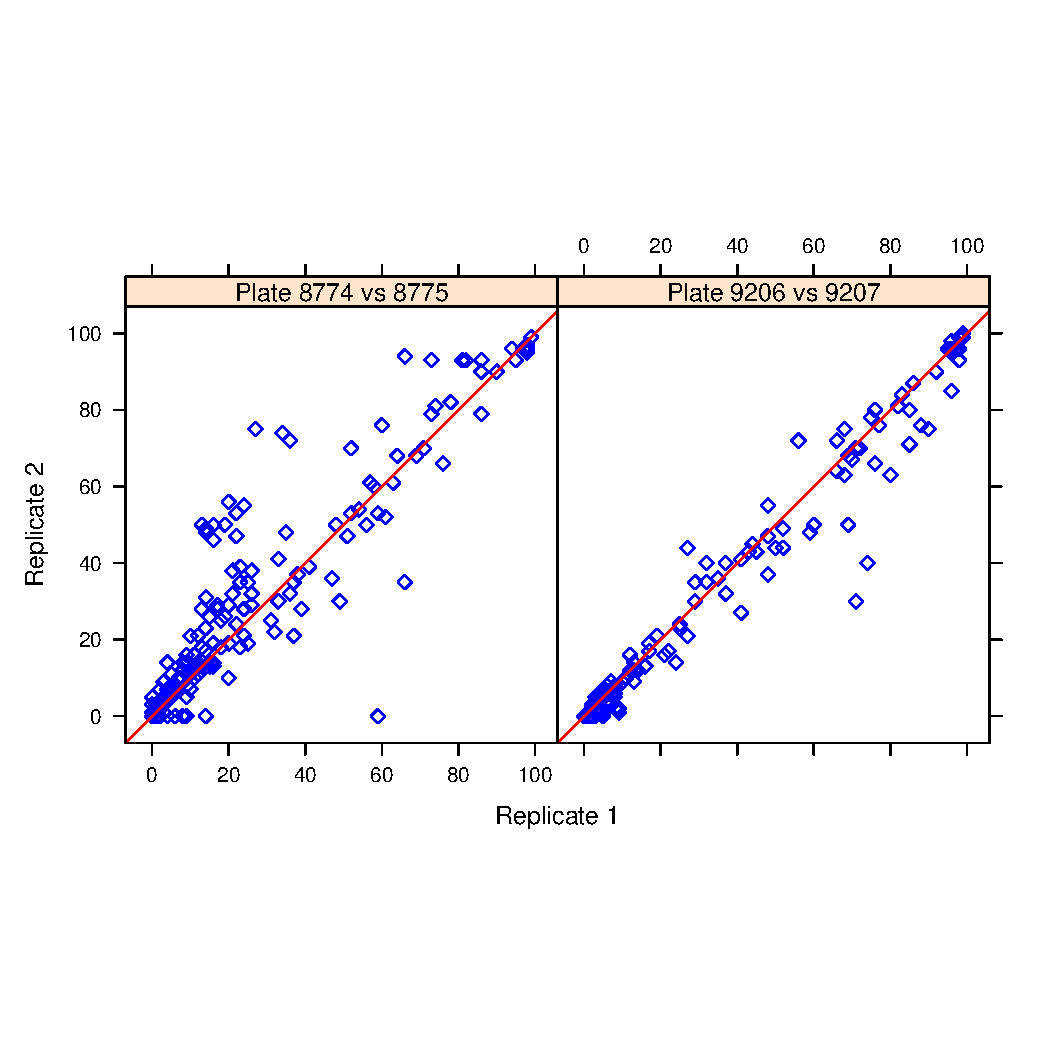
\includegraphics{replicate.pdf}
\caption{Estimates made using FlowJo for the percentage of cells above the
isotype threshold for each marker on replicate plates for donor 1 (8774 vs
8775) and donor 2 (9206 vs 9207). Estimates from markers where the population
of cells was near the isotype threshold, around 50\%, were more
variable than samples which were clearly positive($\ge$99\%) or negative
($\le$1\%). The correlation for replicate plates was strong in both donors, with
donor 1 at 0.92 and donor 2 $\ge$0.98 (plate 9208 for donor 2 not shown).}
\label{fig:replicate}
\end{figure}

\begin{figure}
\centering
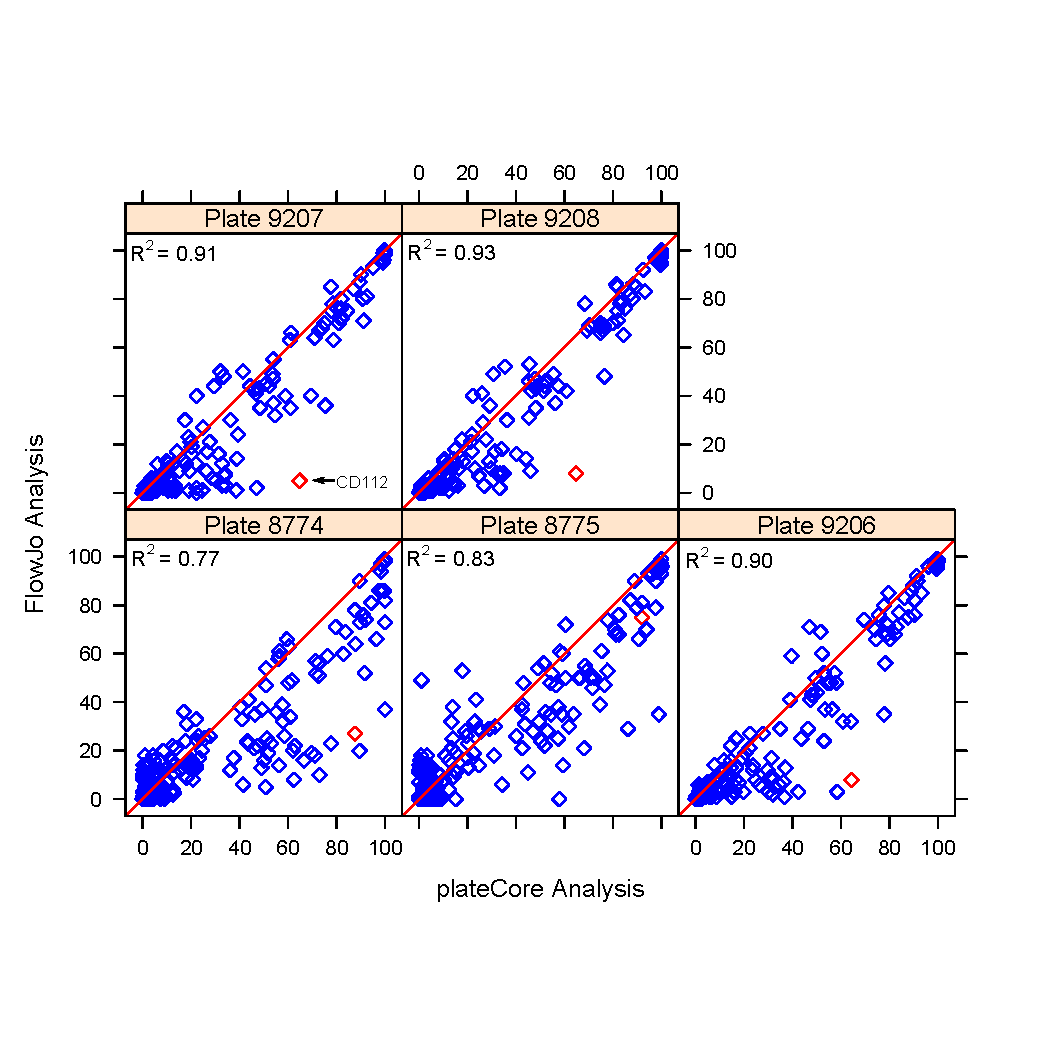
\includegraphics{fjVSr.pdf}
\caption{Percent positive results for 189 BD FACS CAP markers analyzed using
either \Rpackage{plateCore} or FlowJo for the 5 PBMC plates. }
\label{fig:pcVSman}
\end{figure}

\begin{figure}
\centering
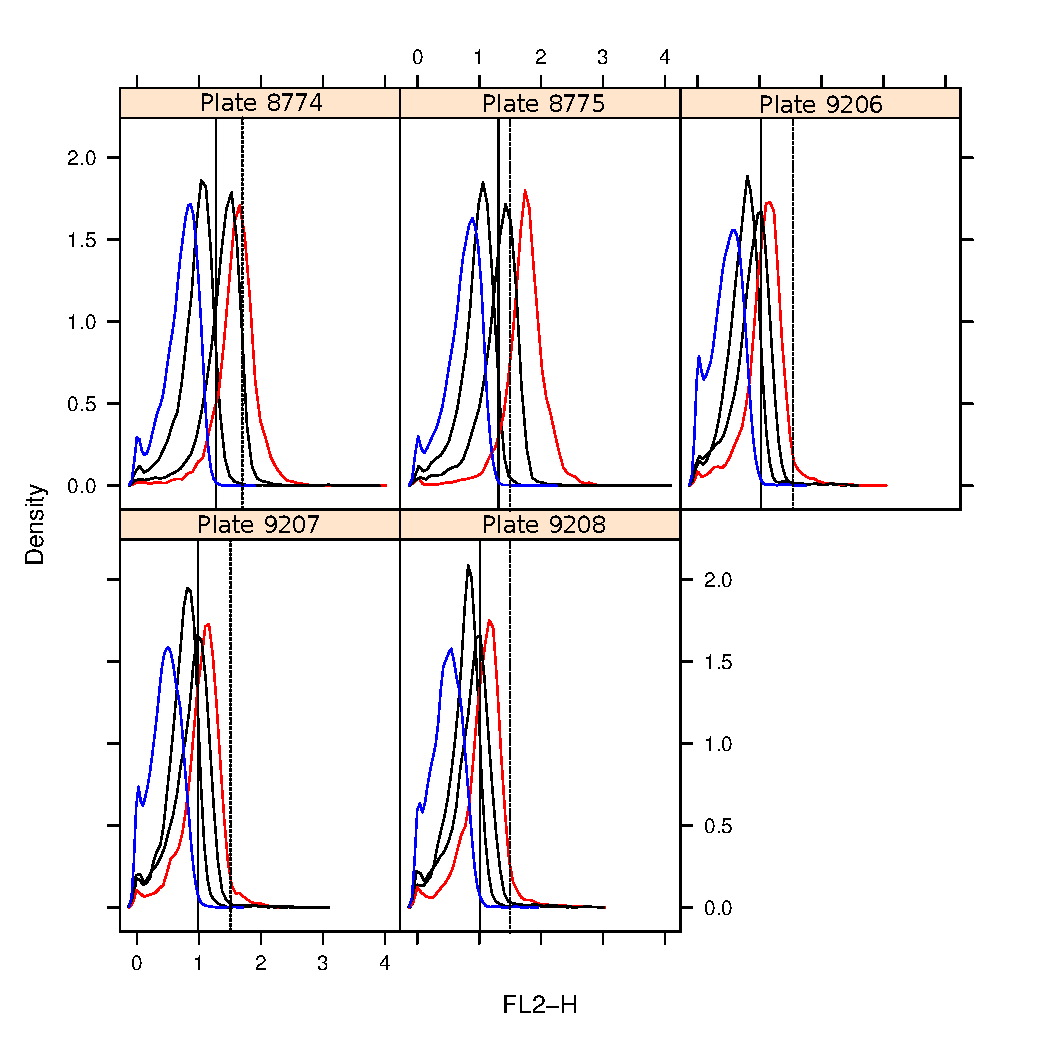
\includegraphics{fjVSr3.pdf}
\caption{CD112}
\label{fig:pcVSman2}
\end{figure}

%%%%%%%%%%%%%%%%%%%%%%%%%%%%%%%%%%%%%%%%%%%%%%%%%%%%%%%%%%%%%%%%%%%%%%%%%%%%%%%
\clearpage
\subsection*{Gating Quality Assessment}

Since we may not always have access to output from expert cytometrists to
help determine if our isotype-based gating is reasonable, we need an alternative
approach to assessing gate quality. The strategy used in \Rpackage{plateCore}
looks at the percentage of cells above the isotype gates versus the Median
Fluorsence Intensity (MFI) ratio to see if the gating was consistent across the
experiment (Figure~\ref{fig:mfiRatio}). The MFI ratio is defined as the ratio
of the median fluoresence signal for a marker divided by the median signal for
its isotype control. Essentially, the MFI ratio tells us how well separated the
stained test sample is from its negative isotype control. 

Figure~\ref{fig:mfiRatio} shows the results of a robust logistic regression for
the percentage of positive cells on the MFI ratio for the 189 markers
from the 5 plates. The bulk of the marker values (927 out of 945) are within 2
standardized residuals from the best fit line, which is surprising since the
different antibodies were conjugated to different fluorophores (either Alexa
488, FITC, PE, PerCP, APC, or Alexa 647) and matched against different isotypes
(either IgG1, IgG2, IgG2a, IgG2b, IgG3, or IgM). The 18 remaining cases were
examined in detail and the isotype gates were reasonble, but there were
multiple populations of cells in the test well (Figure~\ref{fig:mfiRatio3}). 

\begin{figure}
\centering
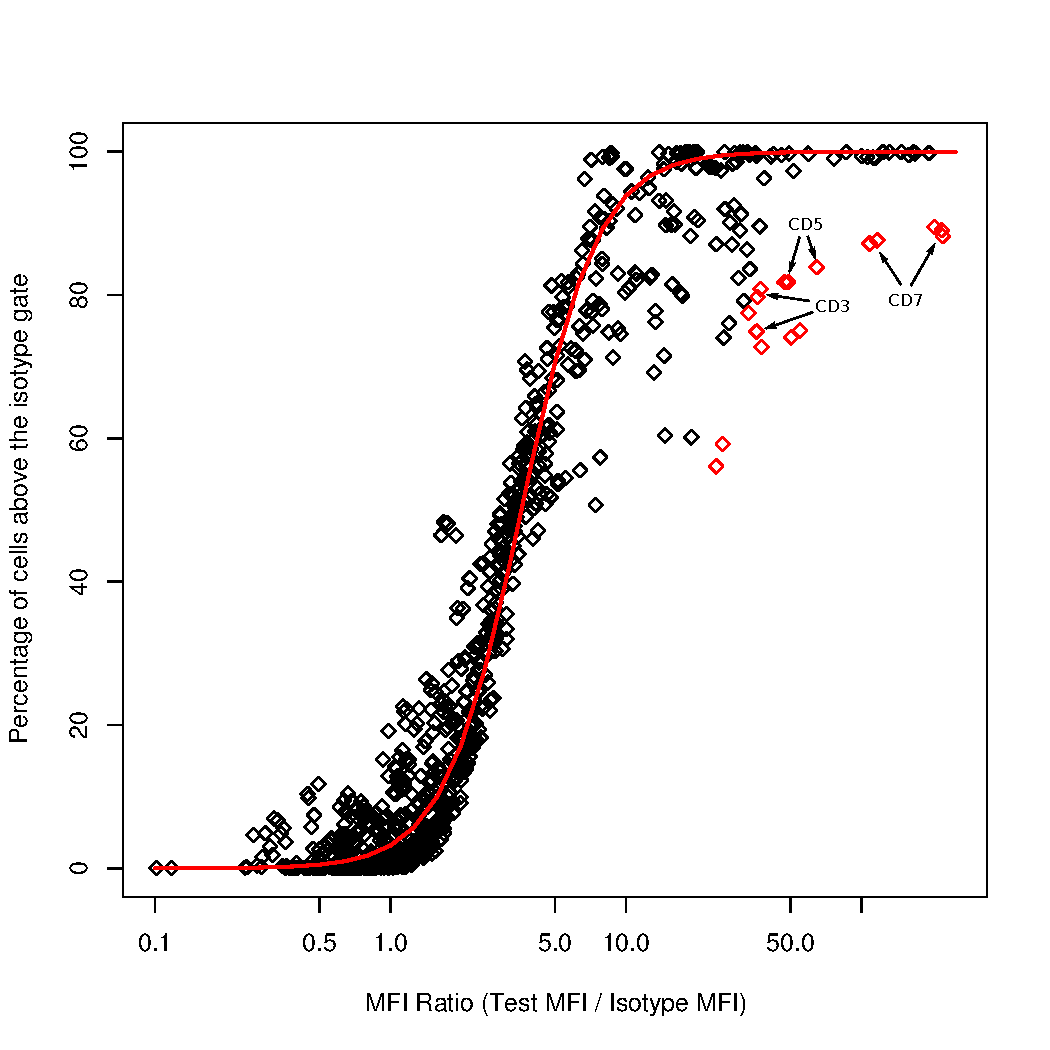
\includegraphics{mfiRatioB.pdf}
\caption{}
\label{fig:mfiRatio}
\end{figure}

\begin{figure}
\centering
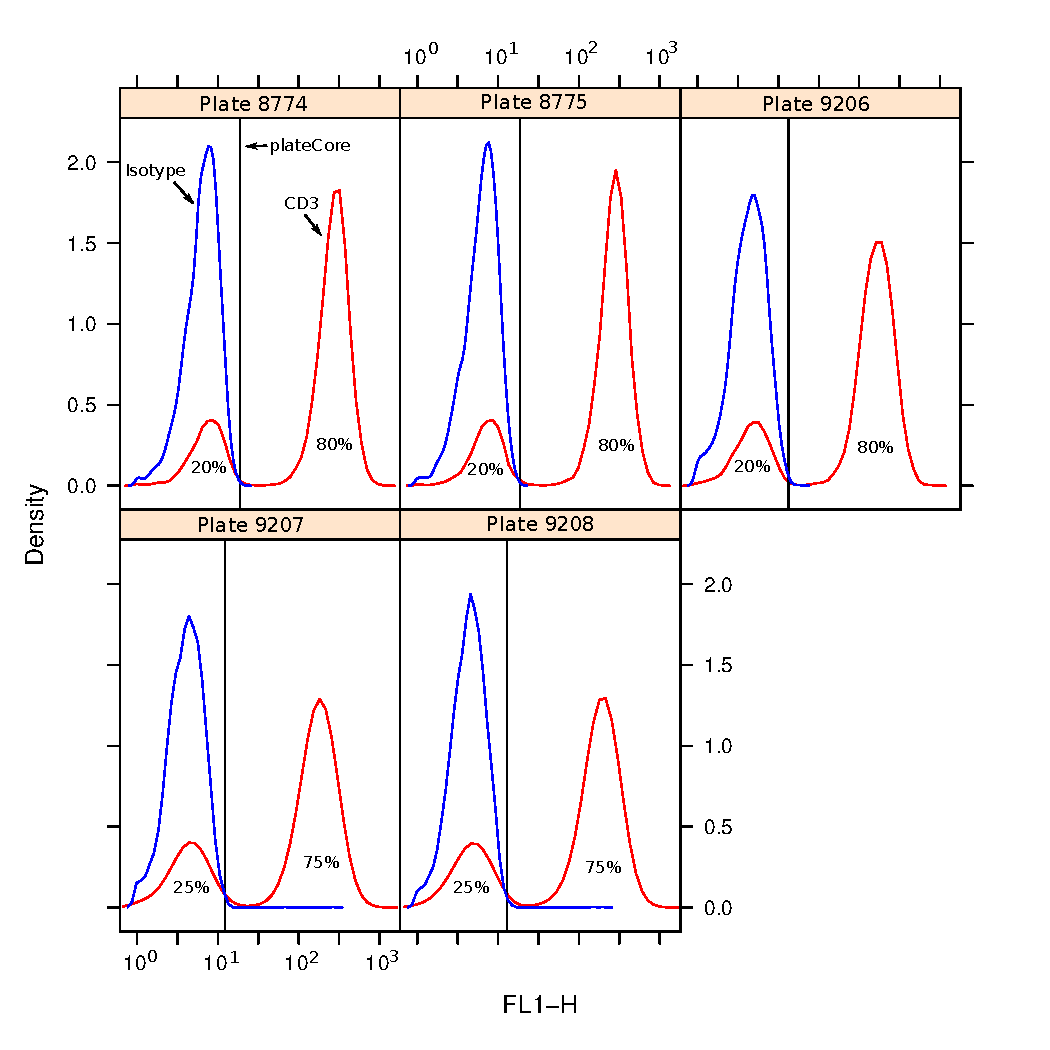
\includegraphics{mfiRatio2.pdf}
\caption{}
\label{fig:mfiRatio3}
\end{figure}

%%%%%%%%%%%%%%%%%%%%%%%%%%%%%%%%%%%%%%%%%%%%%%%%%%%%%%%%%%%%%%%%%%%%%%%%%%%%%%%
\clearpage
\section*{Discussion}

Our approach to this PBMC BD FACS CAP study relied on processing the raw data
in parallel using both FlowJo and \Rpackage{plateCore}. FlowJo allowed the
ctyometrists to thoroughly investigate individual wells, and gave them
confidence that the \Rpackage{plateCore} results were correct (see
Figure~\ref{fig:pcVSman}). Using \Rpackage{plateCore}, we were able to reduce
the level subjectivity in setting isotype gates, eliminate mistakes associated
with manual export and merging of plate output, and automate the creation of
plots and data quality reports that summarized the experiment. Additionally,
the \Rpackage{plateCore} scripts and experimental annotation can be shared with
other cytometry groups, allowing them to reproduce our analysis.

In addition to subjective gating, the lack of a standard format for describing
large FCM experiments also makes it difficult for anyone other than the
original experimenter to replicate an analysis. (You could add something about
MIFlowCyt here as well, as even if people had a format to follow, unless they
put all the data in necessary to understand, just having a format isn't enough
- Ryan) The development of mechanism to bundle experimental metadata
descriptions with FCS data files should make it easier to access metadata in
future FCM studies, but currently this information is typically provided either
as spreadsheet or a pictorial layout of a 96 well plate. Since the creation of
\Robject{flowPlate} requires users to make a standard sample annotation file,
plate layouts from \Rpackage{plateCore} can then be easily shared along with
the raw FCS2.0/3.0 files. The standard format for \Rpackage{plateCore} sample
annotations provides a convenient way to manage the plate metadata associated
with complex FC-HCS experiments.

%moved from methods
While this same analysis can be performed relatively quickly in 
other FCM software packages, it can be difficult to reproduce the gating
decisions made by a single expert user. (Expand - Ryan)

Markers that are expressed on a small subset of lymphocytes, or markers that
are dimly expressed, would not be found with this screening approach.
(Expand - Ryan)

Since, BD FACS CAP was designed as screening tool to 
identify markers for further analysis, false negatives were a bigger concern
than false positives. The plateCore settings were chosen to err on the side of
calling samples positive. (Why, make it clear to uninformed readers by stating
explicitly? what about for other studies? more discussion here - Ryan)

The complexity of large FCM experiments, like BD FACS CAP, highlight the 
difficulty of applying existing FCM analysis platforms to high-throughput
studies. Generating and interpreting results from this PBMC study required
extensive collaboration between flow cytometrists, bioinformaticians, and
statisticians. At various points in the analysis, each group needed to access
the raw data, annotation, and details about the experimental design. Providing
this access using stand-alone FCM platforms is expensive in terms of the price
of multiple software licenses and in time spent training statisticians and
bioinformaticians to use the programs. Fortunately the Bioconductor FCM
packages are modeled on standard data structures used for microarrays, which
should already be familiar to most quantitative individuals working on
high-throughput biological problems. We found that \Rpackage{flowCore},
\Rpackage{flowViz}, and \Rpackage{plateCore} provided an open analysis platform
that facilitated communication between the flow cytometrists generating the
data, and the computational experts analyzing the data.


%%%%%%%%%%%%%%%%%%%%%%%%%%%%%%%%%%%%%%%%%%%%%%%%%%%%%%%%%%%%%%%%%%%%%%%%%%%%%%%
\clearpage
\bibliographystyle{plain}
\bibliography{outline} 

\end{document}
